$subject$=Физические основы компьютерных \\ и сетевых технологий
$teacher$=Лекции Герта А. В.
$date$=31.03.2025

\section{Лекция 8. Волна}

Волна - изменение состояния среди или поля, распространяющееся в пространстве и переносящее с собой энергию.
В случае упругой (механической) волны таким возмущением является деформация среды, движение которой сопровождается
разного рода смещением частиц среды, зависящим от природы волны

Волны можно разделить на два типа: продольные (направления колебаний частиц параллельно с направлением распространением волны) 
и поперечные (направление колебания частиц перпендикулярно направлению распространения волны)

Функция $\xi(x, t)$, описывающая смещение частицы, является решением волнового уравнения:

\[\frac{\partial^2 \xi(x, t)}{\partial x^2} = \frac{1}{v^2} \frac{\partial^2 \xi(x, y)}{dt^2}\]

В каждом случае волна распространяется в среде с определенной скоростью $v$. Эта скорость определяется механическими
свойствами вреды и не то же самое, что скорость движения частиц в волне

Сама среда в целом не перемещается в пространстве, ее частицы движутся вверх-вниз, вперед-назад и так далее относительно положения равновесия

Гармоническая волна - волна, в которой каждая точка совершает гармонические колебания

$\lambda = v T$ - длина волны, расстояние между точками с одинаковыми состояниями (фазами) колебаниями

\smallvspace

\begin{center}
    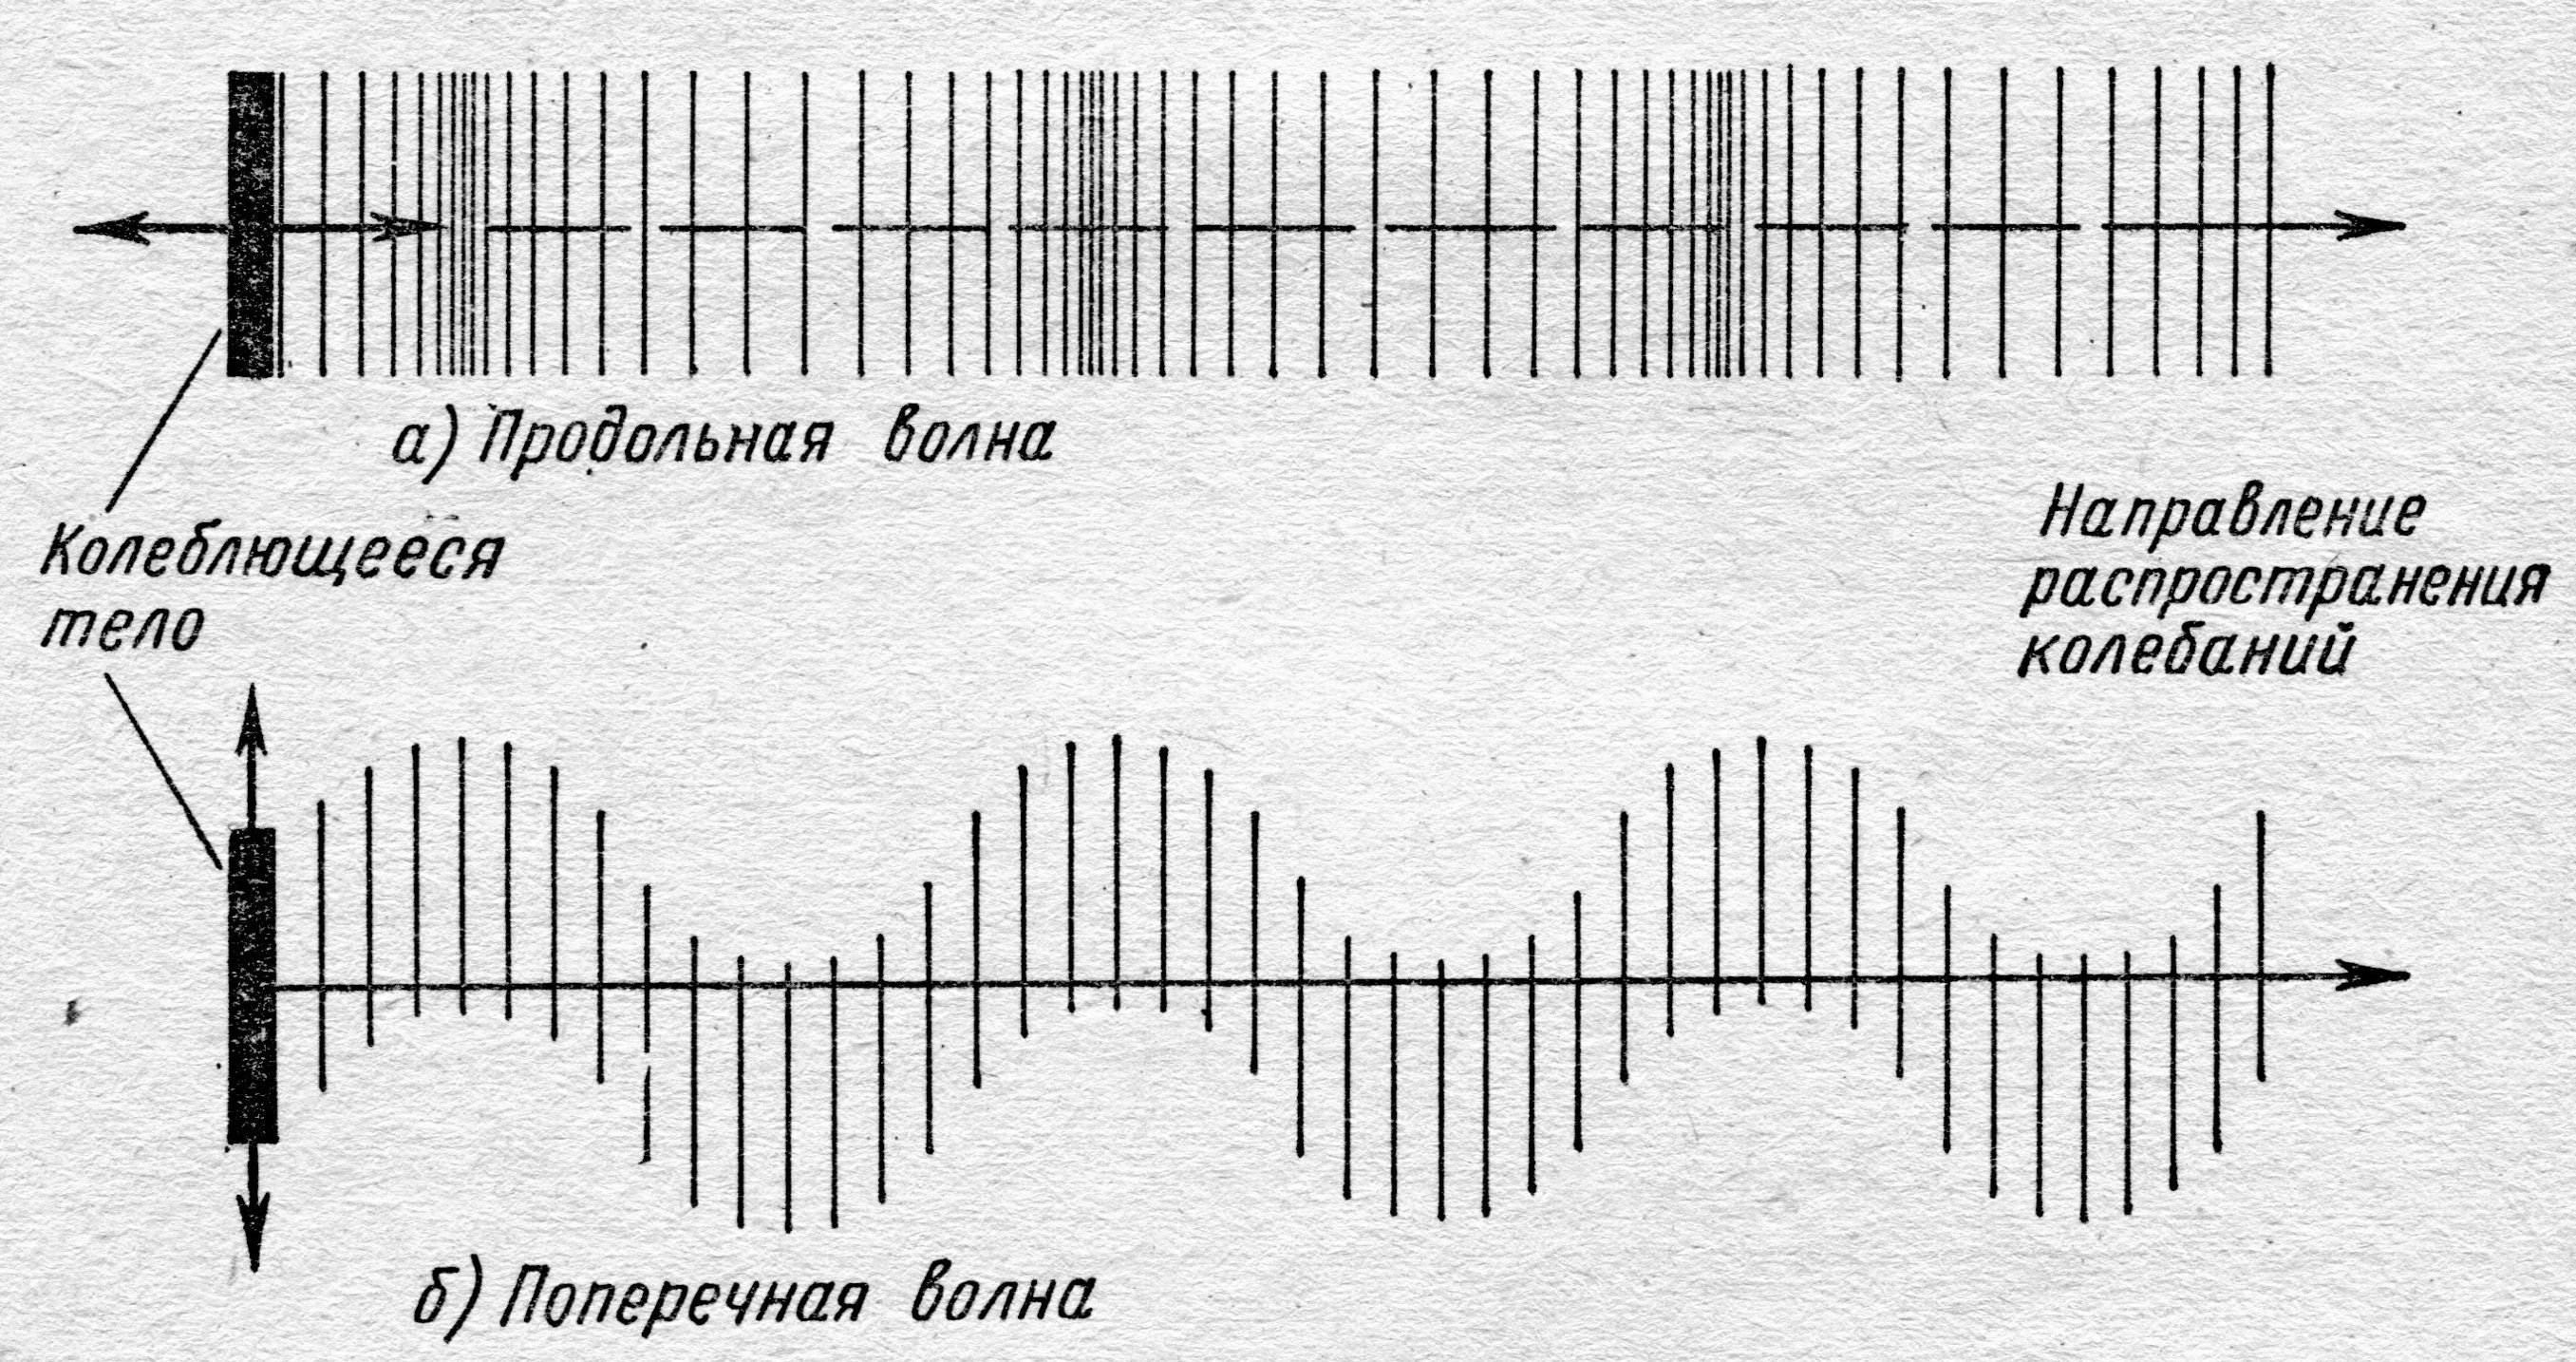
\includegraphics[width=0.75\textwidth]{physics2/images/physics2_2025_03_31_1}
\end{center}

\smallvspace

Аргумент косинус называется фазой $\varphi = \omega t - kx + \varphi_0$

Если зафиксировать значение фазы $\omega t - kx + \varphi_0 = \operatorname{const}$, то это значение с течением
времени перемещается в направлении оси $Ox$ со скоростью, определяемой из условия $\frac{d\varphi}{dt} = \frac{d}{dt} (\omega t - kx + \varphi_0) = 0$

Фронт волны -- это совокупность точек, колеблющихся в одной фазе, до которых в данный момент времени дошел волновой процесс

Волновая поверхность -- поверхность, проведенная через равновесные положения частиц среды, совершающих колебания в одинаковой фазе

Скорость многих механических волн может быть записана в общем виде: 

$v = \sqrt{\frac{\text{возвращающая сила, стремящаяся вернуть систему в состояние равновесия}}{\text{инерция системы, противодействующая этому переходу}}}$

\mediumvspace

Поток энергии - количество энергии, переносимое волной через определенную поверхность за единицу времени: $\Phi = \frac{dW}{dt}$ 

Плотность потока энергии - поток энергии через единичную площадку, перпендикулярную направлению волны: $J = \frac{d\Phi}{dS}$


